
\chapter{Pruebas, validación y resultados}\label{resultados}
Las pruebas y la validación son etapas críticas en el desarrollo de cualquier sistema de software, ya que permiten garantizar que la aplicación cumple con los requisitos funcionales y no funcionales, además de asegurar su correcto funcionamiento en diferentes escenarios. A continuación, se describen las estrategias y metodologías utilizadas para validar el correcto funcionamiento de SIDManager, así como los resultados obtenidos durante este proceso.

\section{Estrategia de pruebas}
Para garantizar la calidad del software, se ha seguido una estrategia de pruebas que combina técnicas de prueba manual y automatizada. Esta estrategia se ha dividido en tres niveles principales:

\begin{itemize}    
    \item \textbf{Pruebas de integración}: Se han llevado a cabo pruebas para validar la interacción entre los diferentes componentes del sistema, como la conexión entre el backend y la base de datos, o la integración entre los servicios y los controladores. Estas pruebas han sido esenciales para detectar posibles errores en la comunicación entre módulos.
    
    \item \textbf{Pruebas de sistema}: Se han realizado pruebas end-to-end para validar el flujo completo de la aplicación, desde la interacción del usuario con la interfaz hasta la persistencia de datos en la base de datos. Estas pruebas han incluido escenarios como el registro de usuarios, la autenticación, la gestión de documentos y la recuperación de contraseñas.
\end{itemize}

\section{Validación de requisitos}
Durante las pruebas, se ha validado que la aplicación cumple con todos los requisitos, incluyendo:

\begin{itemize}
    \item \textbf{Funcionalidades principales}: Registro y autenticación de usuarios, gestión de documentos, filtrado por fechas y verificación del estado de los documentos.
    \item \textbf{Seguridad}: Validación del cifrado de contraseñas y manejo seguro de sesiones.
    \item \textbf{Rendimiento}: Evaluación del tiempo de respuesta de la aplicación bajo diferentes cargas de trabajo, garantizando un rendimiento óptimo incluso con grandes volúmenes de datos.
\end{itemize}


Los resultados obtenidos en el desarrollo de SIDManager demuestran que la aplicación cumple con los objetivos planteados inicialmente, ofreciendo una solución robusta, segura y escalable para la gestión y monitorización de documentos en entornos empresariales. A continuación, se presentan los resultados más relevantes del proyecto, tanto a nivel técnico como funcional.

\section{Resultados técnicos}
\begin{itemize}
    \item \textbf{Arquitectura modular}: La aplicación se ha desarrollado siguiendo una arquitectura basada en capas (vista, controlador, servicio, repositorio), lo que ha facilitado su mantenimiento y escalabilidad.
    \item \textbf{Seguridad implementada}: Se ha logrado un alto nivel de seguridad gracias al uso de Spring Security, el cifrado de contraseñas con BCrypt y la protección contra ataques comunes.
    \item \textbf{Integración de tecnologías modernas}: El uso de Spring Boot, Thymeleaf y JPA ha permitido desarrollar una aplicación eficiente y fácil de mantener.
    \item \textbf{Documentación completa}: El código ha sido documentado utilizando Javadoc, lo que facilita su comprensión y mantenimiento por parte de otros desarrolladores.
\end{itemize}

\section{Resultados funcionales}
\begin{itemize}
    \item \textbf{Gestión de documentos}: La aplicación permite filtrar y visualizar documentos de manera eficiente, verificando su correcto almacenamiento en la base de datos como se puede ver en las figuras \ref{fig:documentsView} y \ref{fig:documentsView_2}.
    \item \textbf{Autenticación y registro}: Los usuarios pueden registrarse, confirmar sus cuentas mediante correo electrónico y autenticarse de manera segura. Para ver la apariencia de la parte del registro consultar la figura \ref{fig:sign_up_view}.
    \item \textbf{Recuperación de contraseñas}: Se ha implementado un sistema seguro para la recuperación de contraseñas, utilizando códigos de confirmación únicos.
    \item \textbf{Interfaz intuitiva}: La interfaz de usuario, desarrollada con Thymeleaf y Bootstrap, es clara y fácil de usar, lo que mejora la experiencia del usuario.
\end{itemize}


\begin{figure}
    \centering
    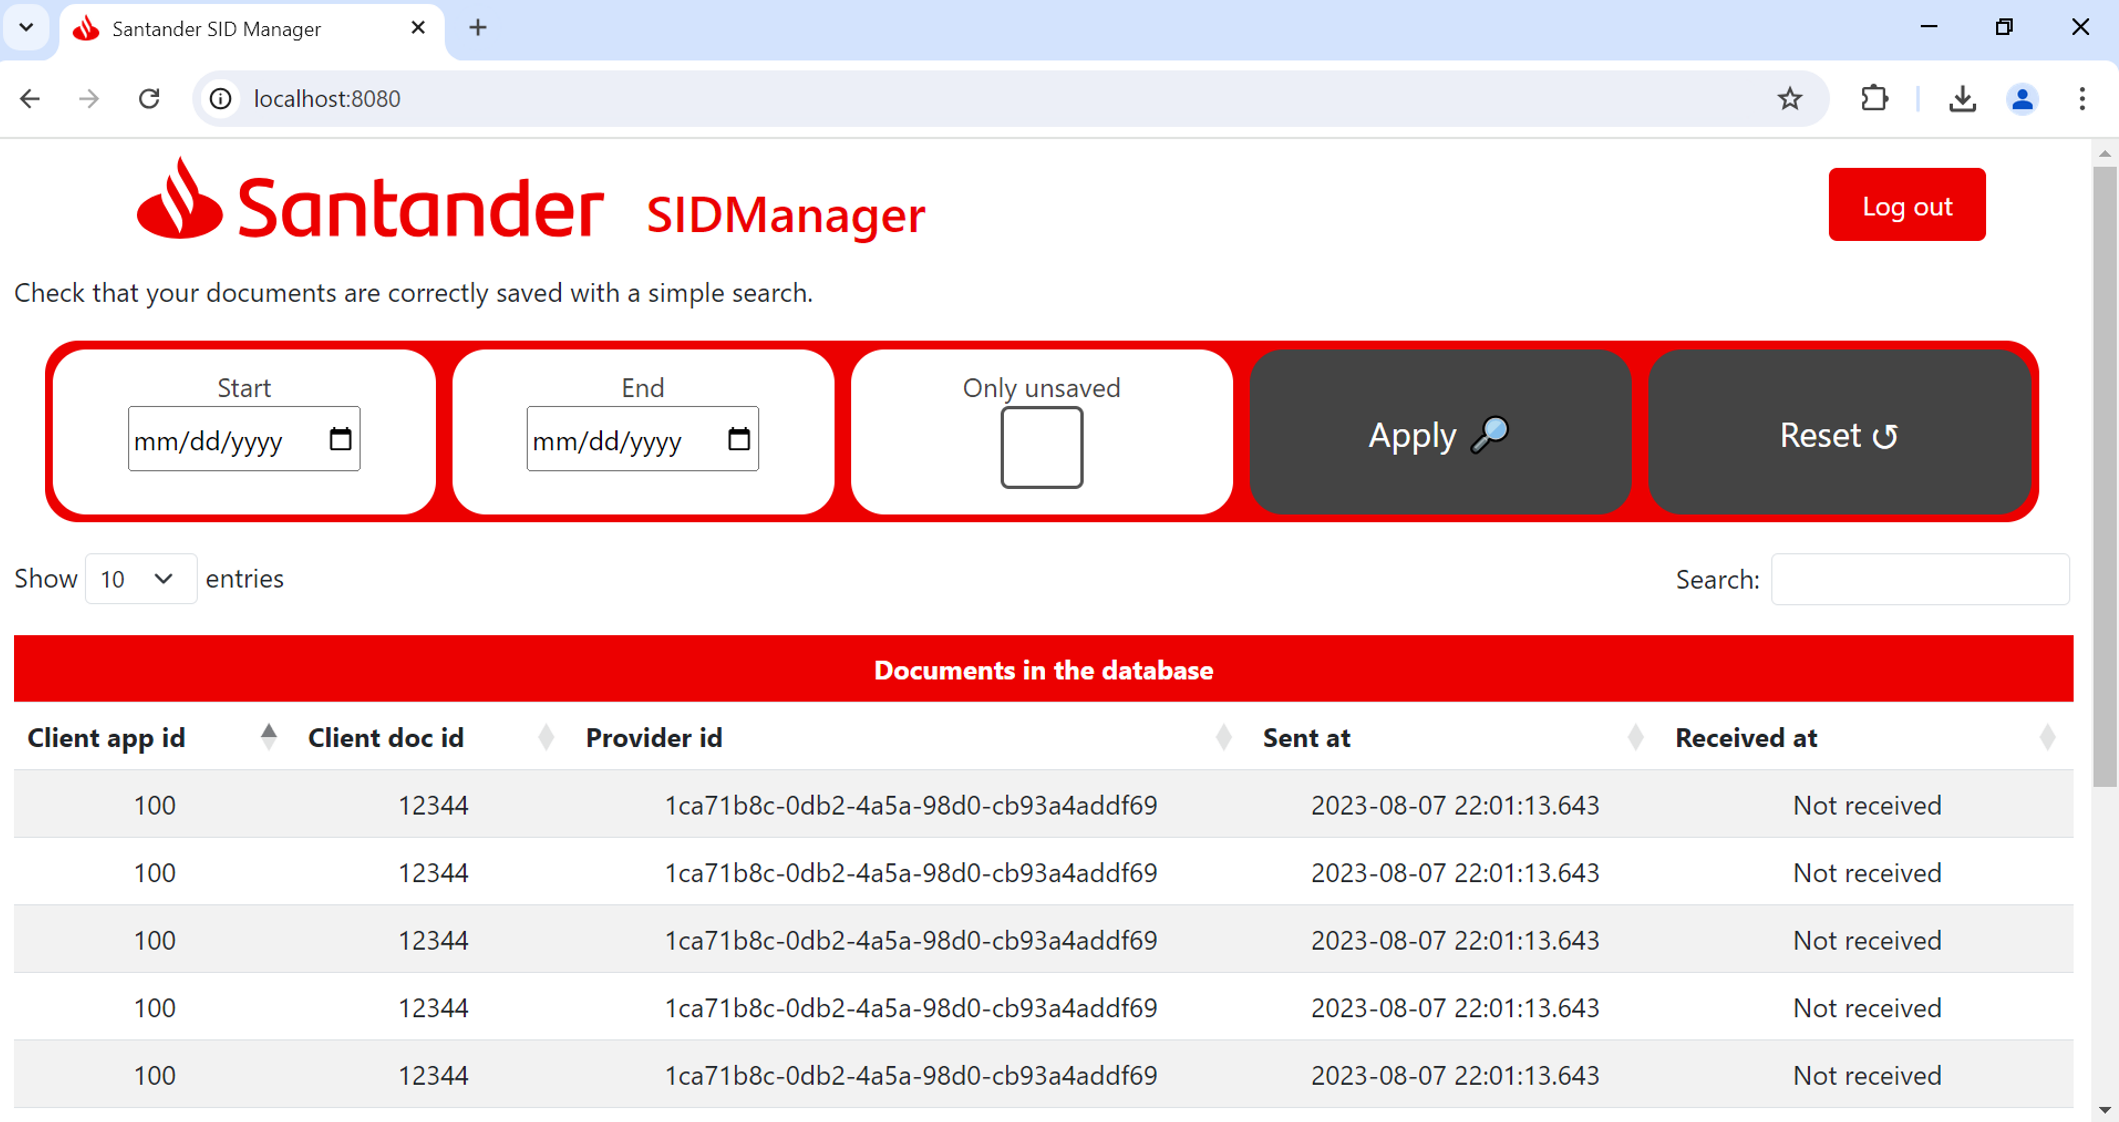
\includegraphics[width=0.75\linewidth]{imagenes/view/documentsView.png}
    \caption{Apariencia de la página principal de la aplicación SDIManager}
    \label{fig:documentsView}
\end{figure}

\begin{figure}
    \centering
    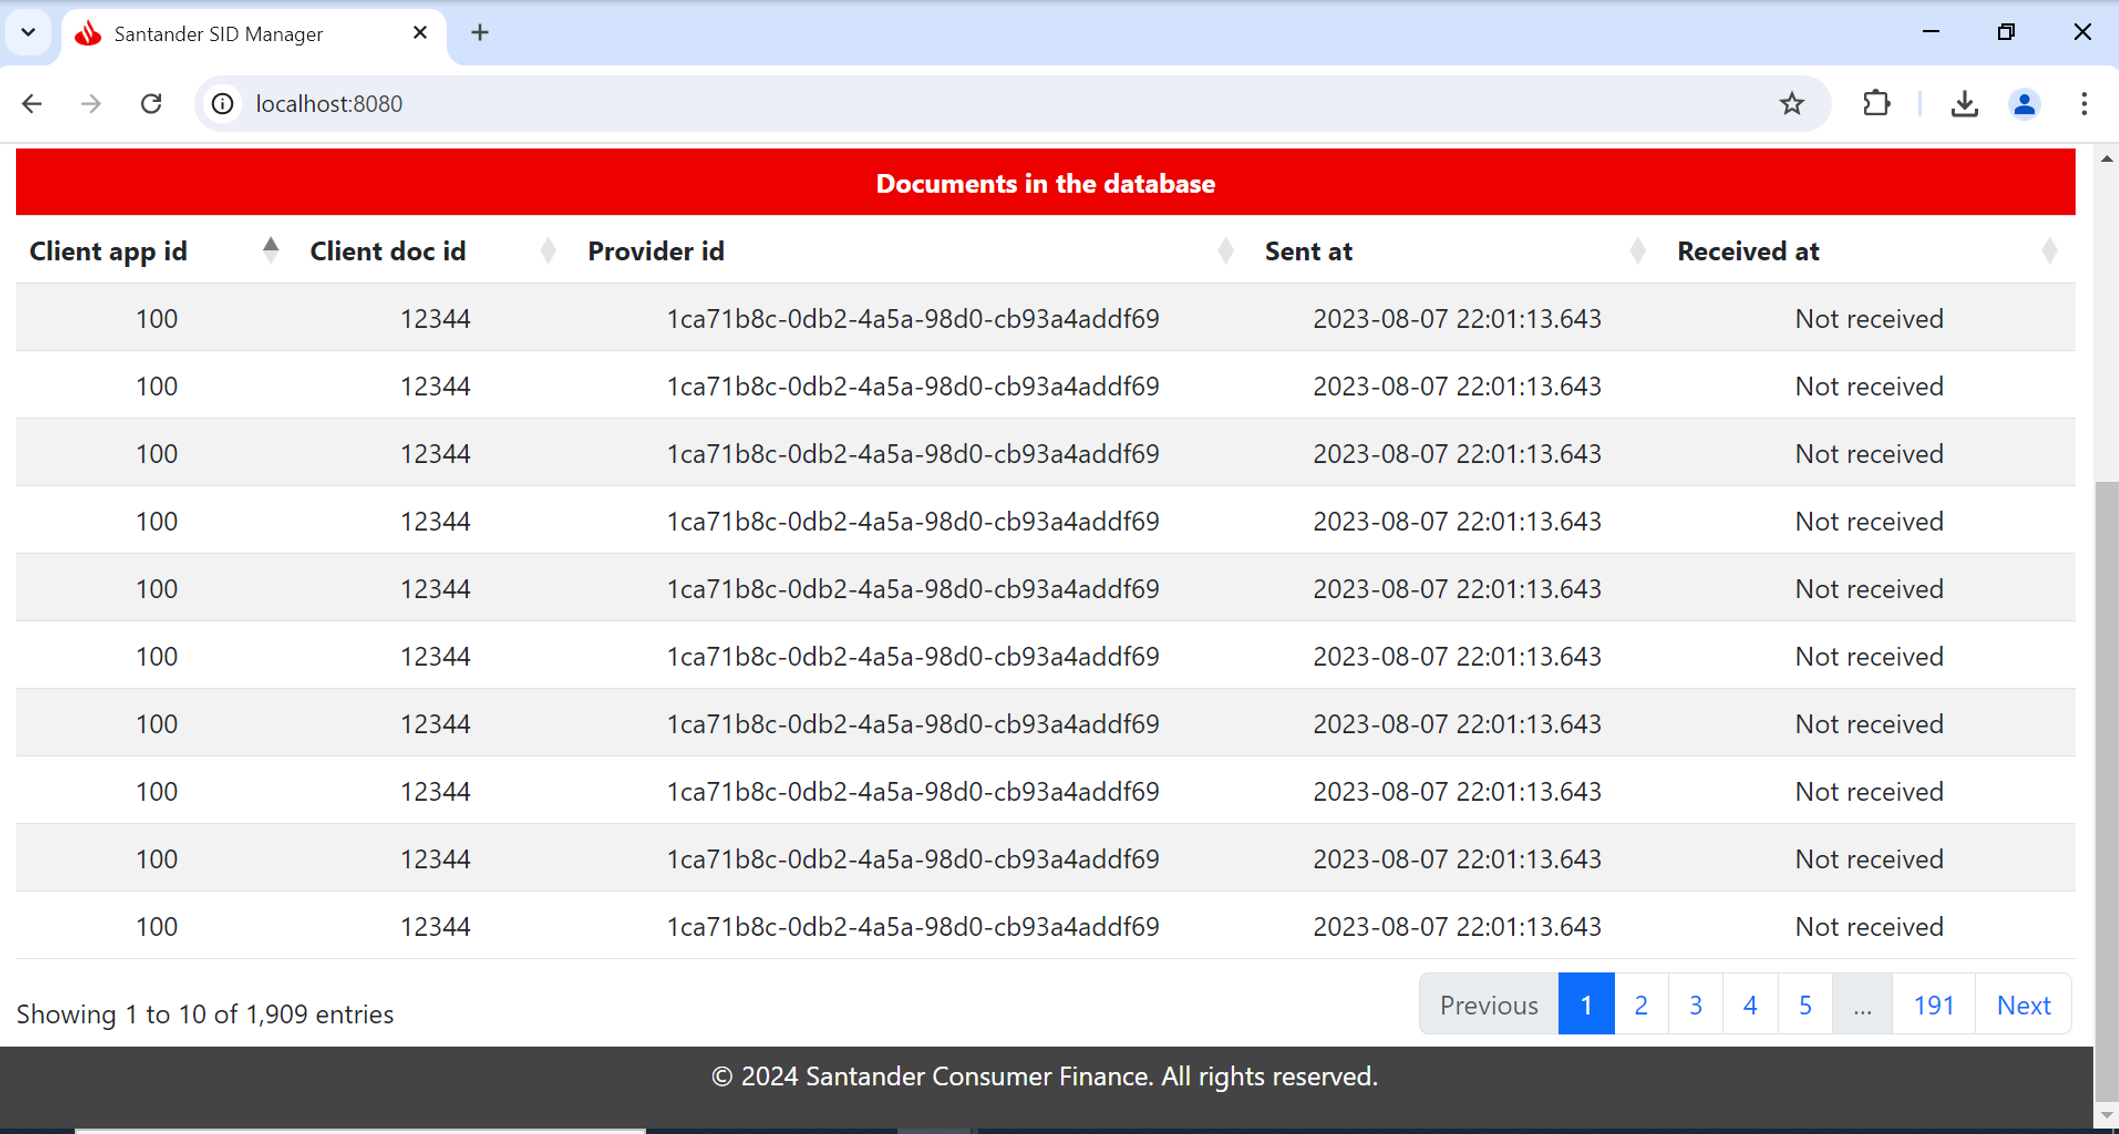
\includegraphics[width=0.75\linewidth]{imagenes/view/documentsView_2.png}
    \caption{Apariencia de la parte baja de página principal de la aplicación SDIManager}
    \label{fig:documentsView_2}
\end{figure}

\begin{figure}
    \centering
    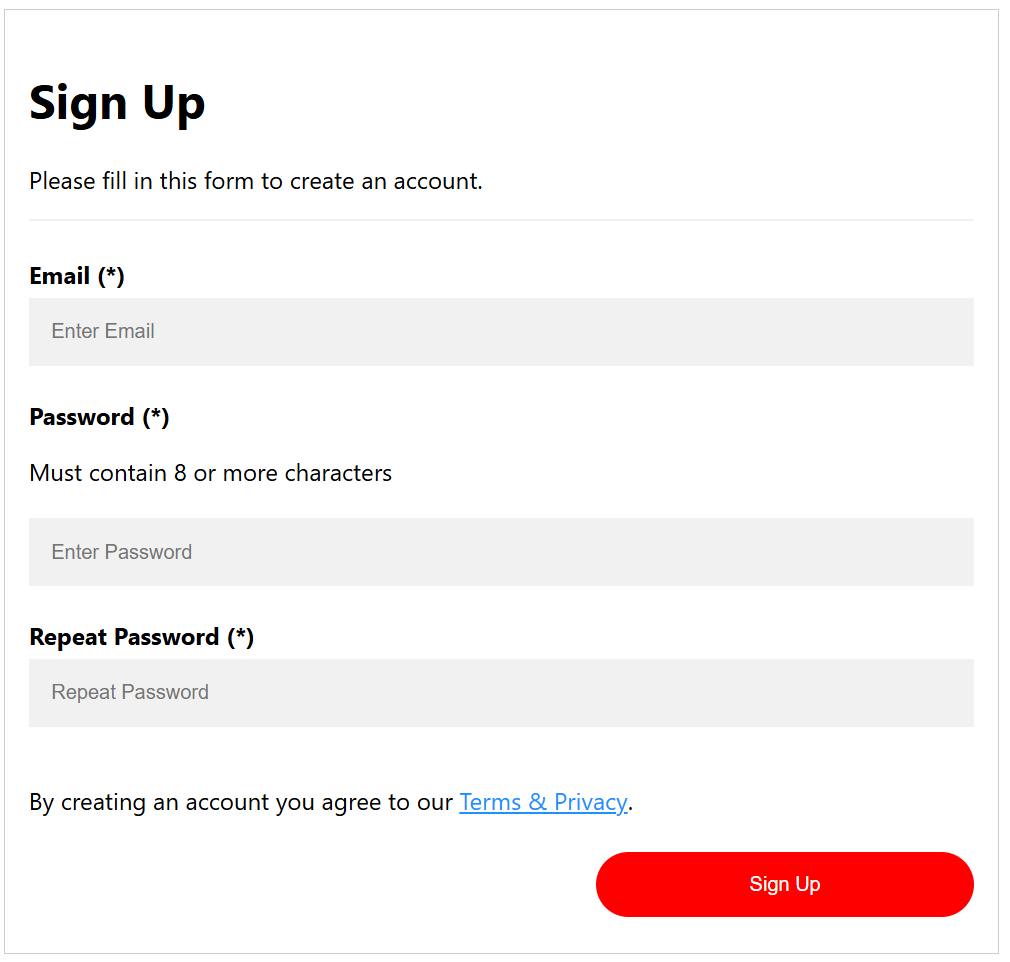
\includegraphics[width=0.75\linewidth]{imagenes/view/sign_up_view.png}
    \caption{Apariencia del registro de usuarios de la aplicación SDIManager}
    \label{fig:sign_up_view}
\end{figure}

Para más información de los resultados y las interfaces finales, se puede visualizar el video sobre la aplicación SIDManager en el siguiente enlace \url{https://youtu.be/DZQm53UCwSE}.